Tracks and their angular resolution could not only improve the jet mass definition but also the performance of tagging variables such as the Energy Correlation Functions or n-Subjettiness. These variables are usually calculated with calorimeter clusters as input, studied here are tracks and assisted tracks as input in comparison with the default method using clusters. 
In contrast to the $\mta$ variable introduced in Section \ref{subsec:mta}, not the mass but the $p_{\mathrm{T}}$ of each track is scaled, since C2, D2, $\tau_{21}$ and $\tau_{32}$ are calculated with the constituents $p_{\mathrm{T}}$.

The concept of track assisting with the $p_{\mathrm{T}}$ ratio of the whole jet is without effect for the studied substructure variables. This can be understood from the definitions of the weighted $p_{\mathrm{T}}$ sums. If corrected with only one ratio, all tracks are scaled by the same factor $c$, which then can be put in front of the sum and cancels as soon as the ratios $\tau_{21}$ and $\tau_{32}$, respectively C2 and D2 are formed.
\begin{equation}
\begin{aligned}
 & \tau_N ={} \frac{1}{d_0}\sum_k p_{T,k} \; c \; min(\Delta R_{1,k},\Delta R_{2,k},...,\Delta R_{N,k})^{\beta} \\
 & \; \; \; \;  ={} \frac{c}{d_0}\sum_k p_{T,k}\:min(\Delta R_{1,k},\Delta R_{2,k},...,\Delta R_{N,k})^{\beta}
\end{aligned}
\end{equation}
Track assisting with ghost association to subjets (TAS), see Section \ref{subsec:mtas} for $\mtas$ works with different scaling factors depending on the corresponding sub-jet $c_k$, which also affect ratios:
\begin{equation}
\tau_N = \frac{1}{d_0}\sum_k p_{T,k} \; c_k \; min(\Delta R_{1,k},\Delta R_{2,k},...,\Delta R_{N,k})^{\beta} 
\end{equation}\label{eq:tas_ta}
This leads to the following adaption of the TAS procedure:
\begin{equation}
\begin{pmatrix}
                    m_{track} \\ p_{T,track} \\ \eta_{track} \\  \phi_{track}
                    \end{pmatrix}       \rightarrow \begin{pmatrix}
                    m_{track}  \\ p_{T,track}  \frac{p_{T,sub-jet}}{\sum\limits_{ga\:tracks}p_{T,track}} \\ \eta_{track} \\ \phi_{track}
            
            \end{pmatrix}  
\end{equation}\label{eq:track_tas}
Where the sum combines the $p_{\mathrm{T}}$ of all tracks that are associated to a given sub-jet. 


\subsection{Event weighting and Mass-Cut}
The substructure variables are compared via their QCD (multi-jet) rejection performance. While the $p_{\mathrm{T}}$ distribution of the multi-jet sample falls exponentially, the $p_{\mathrm{T}}$ of the signal samples features characteristic peaks related to the different resonance masses, see Figure \ref{fig:p_T}. To avoid bias in the comparison, the signal sample is given weights sucht that the truth $p_{\mathrm{T}}$ distribution of the leading jet matches the one of the background sample. Furthermore, the spectrum is split into six different $p_{\mathrm{T}}$ regions to study the behavior with rising energy. 
\begin{figure} 
	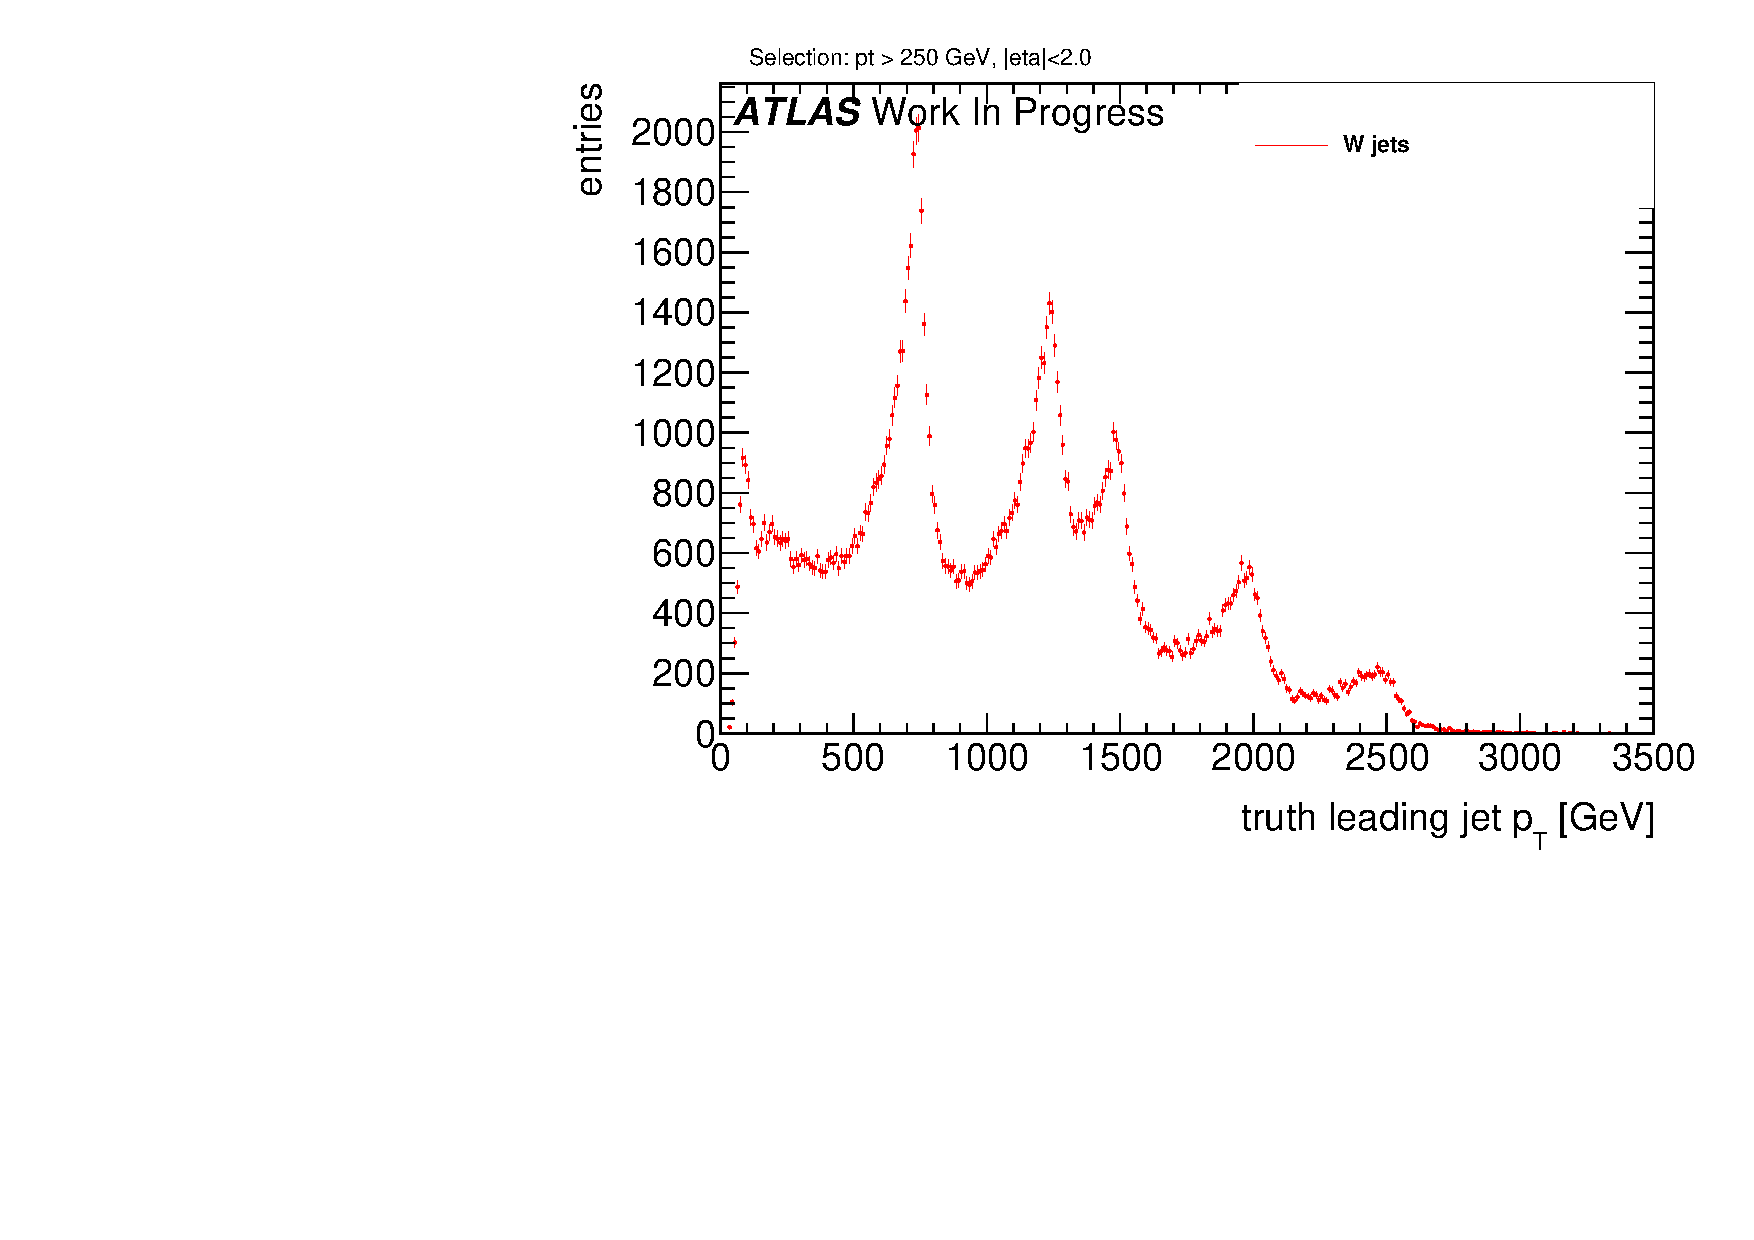
\includegraphics[width=0.5\textwidth]{sascha_input/plots/track_selection/h_leadpt_truth.pdf} \hspace{1mm}
	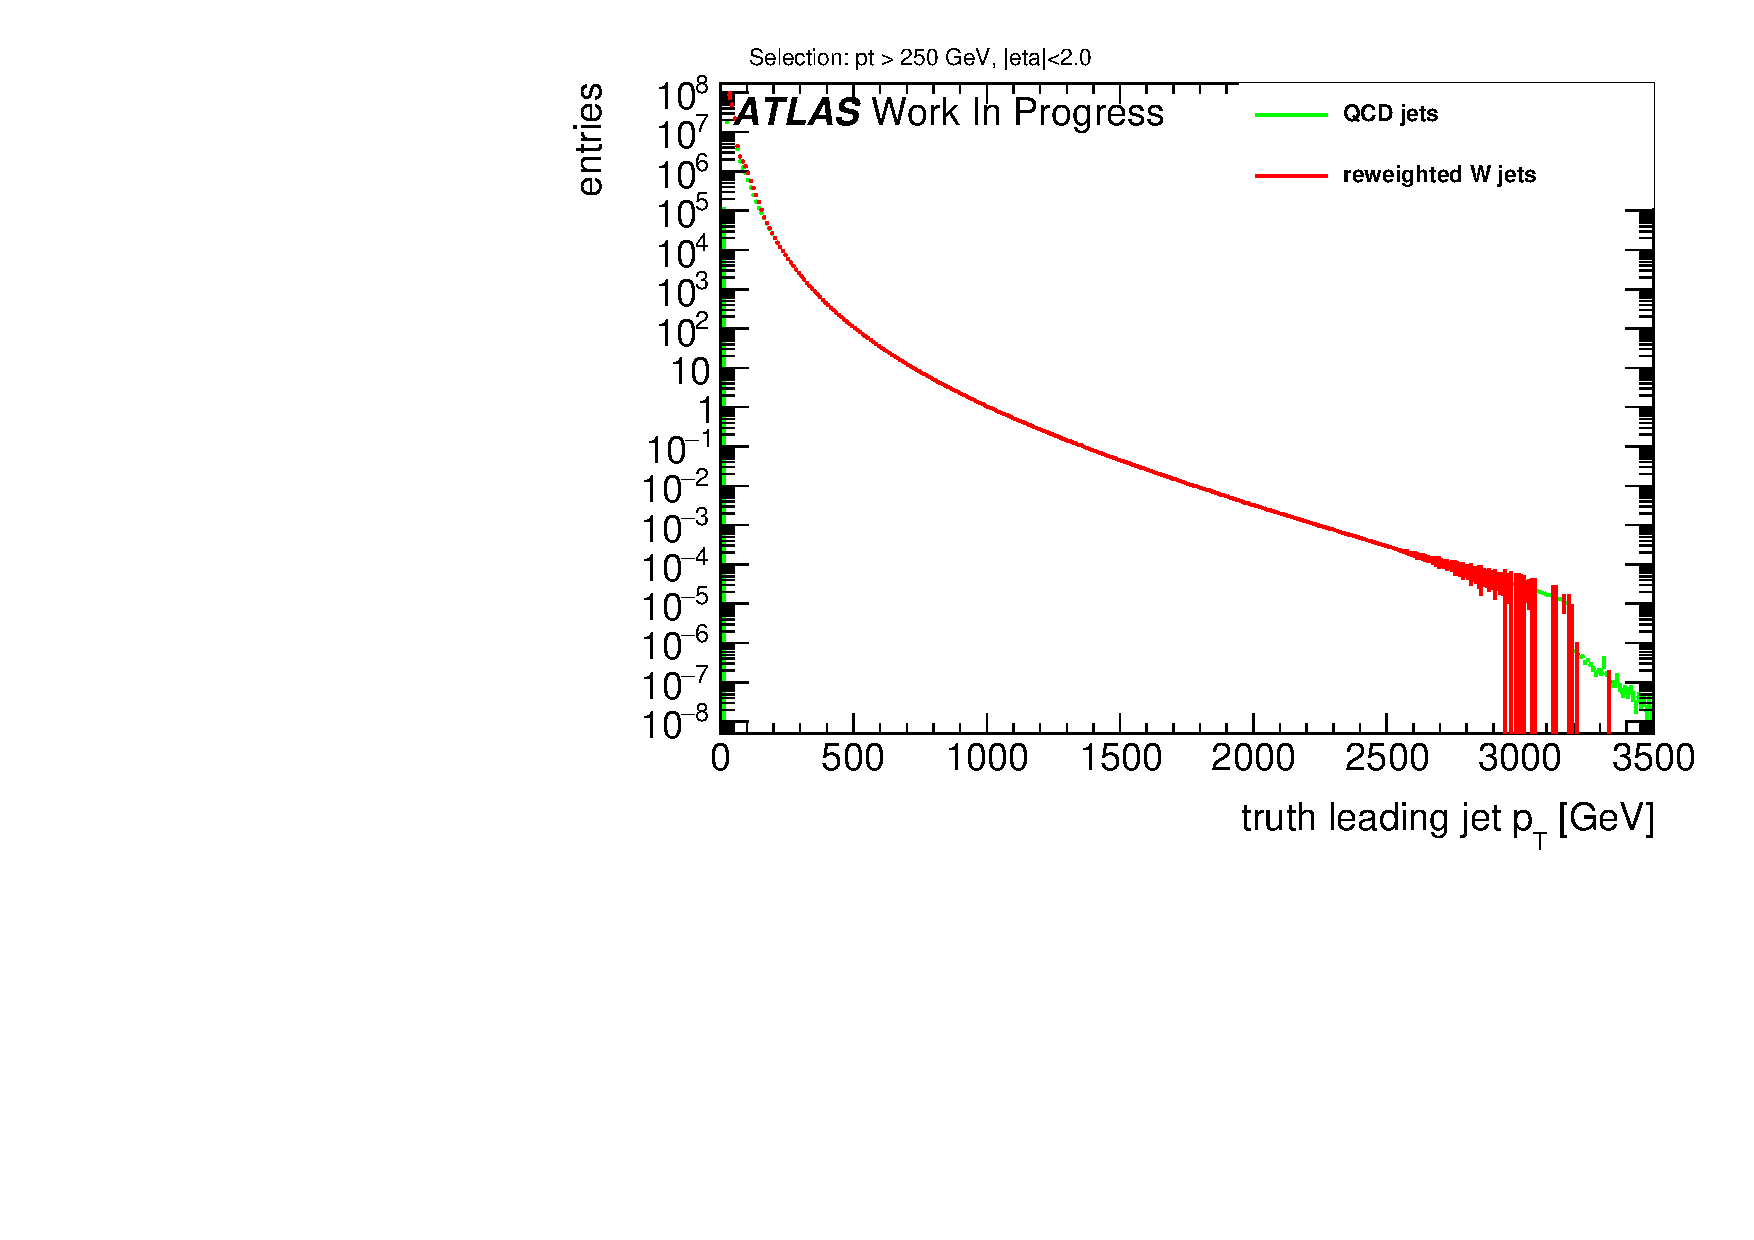
\includegraphics[width=0.5\textwidth]{sascha_input/plots/track_selection/h_leadpt_truth_weight.pdf}
\caption{\footnotesize{Exemplary $p_{\mathrm{T}}$ distributions of (left) $W$ boson jets and (right) QCD jets from multi-jet events with reweighted $W$ boson events}}\label{fig:p_T}
\end{figure}

Tagging variables such as C2, D2, $\tau_{21}$ and $\tau_{32}$ are usually used after applying a mass cut around the interval that contains 68\% of the signal events. Therefore, a cut is applied on the calibrated mass of the large-R calorimeter jet which is calculated to cover the smallest interval around the peak mass that contains 68\% of the signal events.
The comparison is performed in six different $p_{\mathrm{T}}$ regions to study the behavior connected with rising energy of the decaying particle. These regions are presented in the left part of Table \ref{table:mass_cut}. 
In case of the Higgs boson study, there is not enough statistics to derive a conclusive result for $p_{\mathrm{T}} > 2000 \, \text{GeV}$, since the highest resonance mass of the $G^* \rightarrow HH$ samples is $3000 \, \text{GeV}$ in contrast to $5000 \, \text{GeV}$ for the $Z^\prime \rightarrow tt$ and $W^\prime \rightarrow WZ$ samples. Hence this study is restricted to the five lower $p_{\mathrm{T}}$ bins.
Prior to tagging with the n-Subjettiness or C2/D2 variables, a cut on the calibrated calorimeter jet mass is applied, given that the mass is the main discriminant in QCD jet rejection. This cut is defined to choose the smallest interval around the peak mass containing 68\% of the signal. However, the reconstructed mass depends on the $p_{\mathrm{T}}$ region, therefore a different cut was calculated for every region to meet the requirements.
\begin{table}[]
\centering
\begin{tabular}{l||ll||ll||ll}
  &  \textbf{W boson}                                                    &                                 &  \textbf{Higgs boson}                                  &                                &    \textbf{Top quark}                                  &                                  \\ \hline
$p_{\mathrm{T}} \, \text{[GeV]}$   & \multicolumn{1}{l|}{Mass [GeV]} & $\frac{1}{\epsilon_{bgr}}$ & \multicolumn{1}{l|}{Mass [GeV]} & $\frac{1}{\epsilon_{bgr}}$ & \multicolumn{1}{l|}{Mass [GeV]}  & $\frac{1}{\epsilon_{bgr}}$ \\ \hline \hline
250 - 500 & \multicolumn{1}{l|}{63 - 85}                        & 10.8                            & \multicolumn{1}{l|}{56 - 167}          & 3.8                             & \multicolumn{1}{l|}{77 - 191}          & 6.3                             \\ \cline{1-7} 
500 - 800 & \multicolumn{1}{l|}{72 - 92}                        & 13.6                            & \multicolumn{1}{l|}{92 - 150}          & 7.3                             & \multicolumn{1}{l|}{117 -205}          & 6.9                             \\ \cline{1-7} 
800 - 1200 & \multicolumn{1}{l|}{76 - 104}                       & 9.6                             & \multicolumn{1}{l|}{98 - 143}          & 9.5                             & \multicolumn{1}{l|}{122 - 218}         & 6.5                             \\ \cline{1-7} 
1200 - 1600 & \multicolumn{1}{l|}{77 - 107}                       & 7.3                             & \multicolumn{1}{l|}{103 - 149}         & 9.0                             & \multicolumn{1}{l|}{122 - 227}         & 6.3                             \\ \cline{1-7} 
1600 - 2000 & \multicolumn{1}{l|}{79 - 115}                       & 5.6                             & \multicolumn{1}{l|}{91 - 170}          & 4.4                             & \multicolumn{1}{l|}{121 - 235}         & 5.6                             \\ \cline{1-7} 
$> 2000$ & \multicolumn{1}{l|}{80 - 126}                       & 4.2                             & \multicolumn{1}{l|}{/}                 & /                               & \multicolumn{1}{l|}{123 - 251}         & 4.8                             \\ \hline
\end{tabular}
\caption{\footnotesize{Studied $p_{\mathrm{T}}$ regions and corresponding calculated 68\% mass intervals along with the background rejections from the mass cut for $W$ boson, Higgs boson and Top quark jets.}} \label{table:mass_cut}
\end{table} 


